\scanpage{22}
\mspage{21}

\begin{center}$-\ 9\ -$\end{center}\hfill n\textsuperscript{o} 276

\uline{Remarque} -- La réciproque du corollaire précédent est fausse ; cf. Exerc. N.

4. -- \uline{Modules filtrés complets}.

Soit $(E,E_n)$ un module filtré sur un anneau filtré $(A,A_n)$. Puisque la structure uniforme du groupe topologique $E$ est définie par un seul écart, il est clair que $E$ \uline{est complet si et seulement si toute suite de Cauchy, dans} $E$ \uline{est convergente}. Par ailleurs en vertu de l'inégalité
\[
d(x_p,x_q)\leqslant\underset{p\leqslant n\leqslant q-1}{\operatorname{Max}}d(x_n,x_{n+1}),
\]
on voit qu'une suite $(x_n)$ de points de $E$ vérifie le critère de Cauchy si et seulement si la suite $d(x_n,x_{n+1})$ tend vers $0$, i.e. si et seulement si la suite de terme général $y_n=x_{n+1}-x_n$ tend vers $0$ dans $E$. On en déduit :

PROPOSITION 4 -- \uline{Pour que le module filtré} $E$ \uline{soit complet, il faut et il suffit que toute série d'éléments de} $E$ \uline{dont le terme général tend vers} $0$ \uline{soit convergente}.

\uline{Corollaire} 1-- \uline{Soit} $(E,E_n)$ \uline{un module filtré complet}. \uline{Tout sous-module fermé de} $E$, \uline{muni de la filtration induite, est complet}. \uline{Tout module quotient de} $E$, \uline{muni de la filtration quotient est complet}.
\margin{\unsure{fait général} pour les top\unsure{.} métrisables\quad !\quad\figure{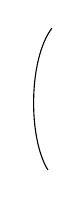
\begin{tikzpicture}[x=1cm,y=1cm]\draw (0.2,0.9) .. controls (-0.1,0.5) and (-0.1,-0.5) .. (0.15,-0.9);\end{tikzpicture}}}

L'assertion concernant les sous-modules \uline{résulte} trivialement de la Proposition. D'autre part, si l'on considère, dans un module quotient $E/F$ une série dont le terme général tend vers $0$, il est clair que celle-ci est l'image d'une série dans $E$ dont le terme général tend vers $0$, donc d'une série convergente dans $E$ ; l'application canonique $E\to E/F$ étant continue, $E/F$ est complet d'après la proposition 1.

\uline{Corollaire} 2 -- \uline{Soient} $(A,A_n)$ \uline{un anneau filtré et complet}, $E$ \uline{un} $A$-\uline{module de type fini}, \uline{filtré par les sous-groupes} $A_nE$. \uline{Alors} $E$ \uline{est complet}

Ecrivons $E=L/R$ où $L$ est un $A$-module libre de type fini ; la filtration de $E$ par les $A_nE$ se déduit alors de la filtration analogue de $L$ ;
